\section{Architektur}{
	Die Architektur wurde inhaltlich so aufgeteilt, dass eine modulare Implementierung möglich ist. So wurden die vier folgenden Bereiche definiert: Persistenz, Applikation, TSP und ACO
	
	Der Begriff der Persistenz beschreibt in diesem Fall zusätzlich zum dauerhaften Abspeichern der Daten, auch das Einlesen der verschiedenen Problemstellungen.
	\newline
	Applikation umfasst den Teil des Programms, der sich nicht direkt mit Daten befasst aber auch nicht zur Problemlösung beiträgt, wie die zwei folgenden Bereiche.
	\newline
	Innerhalb des Begriffs TSP werden alle nötigen Parameter und Methoden behandelt, die basierend auf dem Traveling Salesman Problem notwendig werden. 
	\newline
	Zuletzt gibt es in der Architektur noch das Feld ACO, welches die komplette Berechnung des zu lösenden Problems übernimmt. In dem Fall, dieser Arbeit handelt es sich um das TSP. Allerdings könnte das Problemfeld auch dadurch ausgewechselt werden, dass der Bereich TSP um das neue Problem ersetzt wird.
	
	\subsection{Persistenz}
	Um ein starres Definieren des Problems innerhalb der Applikation zu verhindern, werden zu Beginn des Programms alle Parameter, wie Städtematrix, Wahrscheinlichkeiten und Lösungsparameter aus einer gegebenen XML-Datei eingelesen. Durch eine Bearbeitung der XML ist ein einfaches Abändern der Problemstellung möglich. Hierdurch ist auch gesichert, dass die Algorithmen effizient getestet werden können, da mehrere verschiedenen bekannte Testwerte benannt werden können.
	
	\subsection{Applikation}
	Wie bereits genannt, liegt bei der vorliegenden Architektur ein Fokus auf Modularität, Portabilität und Usability. Aber auch auf verlässliche und effiziente Algorithmen muss geachtet werden. Daher wird für die Wahrscheinlichkeitsberechnung die externe Klasse MersenneTwisterFast \footnote{s. http://www.math.sci.hiroshima-u.ac.jp/~m-mat/MT/emt.html} genutzt, welche eine bessere Distribution der Pseudozufallszahlen bieten als die Default-Implementierung in Java.
	\footnote{Um eine einfache und schnelle Benutzung zu gewährleisten, wird in dieser Arbeit darauf verzichtet echte Zufallszahlen zu nutzen, die beispielsweise aus Weltallstrahlung berechnet werden. Diese seien hier nur zur Vollständigkeit halber erwähnt.}
	Ein weiterer Bestandteil des Applikationsbereichs werden das Logging der Arbeitsvorgänge, sowie die zentrale Konfiguration der Problemstellung auf der die Lösung basiert.
	
	\subsection{TSP}
	Der Bereich des TSP definiert sich in dieser Architektur rein durch die Städte-Objekte, welche zur Darstellung der Städtematrix genutzt werden. Der einzige andere Bestandteil ist die zentrale Aufstellung der Städtematrix, die von den restlichen Klassen nur kopiert wird.
	
	\subsection{ACO}
	Um den Ameisenalgorithmus umzusetzen sind deutlich mehr Aufwände nötig, als zur Darstellung des TSP. Hier werden mindestens eine Ameisenkolonie benötigt \footnote{Die Architektur würde bei ausreichenden Systemressourcen auch eine parallele Berechnung mehrerer Städtematrizen erlauben},
	sowie je Kolonie mehrere Ameisen.
	\newline
	Die Ameisen werden in der Applikation als einzelne Threads gestartet, die über eine CyclicBarrier kontrolliert werden. Dies erlaubt ein möglichst effizientes Parallelisieren der Lösung.
	
	\subsection{Arbeitsweise der Architektur}
	Die einzelnen Abschnitte der Architektur wurden bereits erklärt. Aber das Zusammenspiel der einzelnen Komponenten und der eigentliche Arbeitsablauf des Systems wurde noch nicht beschrieben. Im Folgenden wird ein Beispiel so durchgeführt, wie es auch die geplante Architektur umsetzen würden.
	\begin{figure}[h]
		\centering
		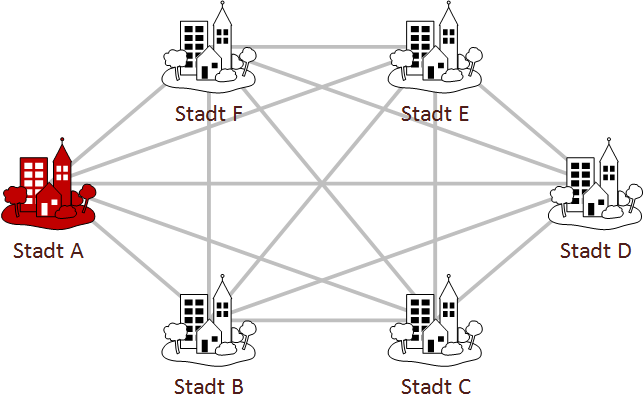
\includegraphics[width=0.9\linewidth]{images/TSP_ACO_numerisch.png}
		\caption{Darstellung des TSP-Beispiels zur Darlegung der Arbeitsweise der Architektur}
		\label{tspAcoNumerisch}
	\end{figure}
}